\section{Evaluation}
\label{sec:evaluation}	

The RDebug algorithm have been evaluated on 3500 MHz Intel(R) Core(TM) i7-2600 CPU workstations
connected by 1 GBit/sec switched Ethernet running Ubuntu 14.04. Each node has 16 GB of main memory.
The experiment results were achieved with 1, 2, 4 and 8 servers on DistGeo platform.

The experiments were performed using three datasets with different characteristics.
The first contains 1000000 points of business listings and points of interest (POIs) from SimpleGeo\footnote{https://github.com/simplegeo}.
The second dataset comprises 226964 lines representing the rivers on Brazil from LAPIG\footnote{www.lapig.iesa.ufg.br}. 
The third contains 220000 polygons of the census of USA from TIGER/Line\footnote{Census 2007 Tiger/Line data}.

The RDebug was executed on DistGeo platform after the indexing of each dataset.
The algorithm was able to collect information about the R-Tree index, such as dead space and overlapping area.
Furthermore, RDebug algorithm has succeeded to collect the index structure allowing visualize each data set R-Tree index on RDebug Visualizer tool.

Three inconsistencies were deliberately inserted in the index to evaluate the RDebug: 
i) inconsistencies between parent and child nodes bounding, ii) nodes filled with more than $M$ entries and iii) duplication of a node on R-Tree. 
The RDebug algorithm was able to identify this inconsistencies in every distributed R-Tree related to datasets. 
The replica consistency on DistGeo is provided by Apache Cassandra \cite{cassandra1apache} and no replica inconsistencies was found in any test. 

\begin{figure}[h]
  \centering
  \subfigure[Node inconsistency]
  {
  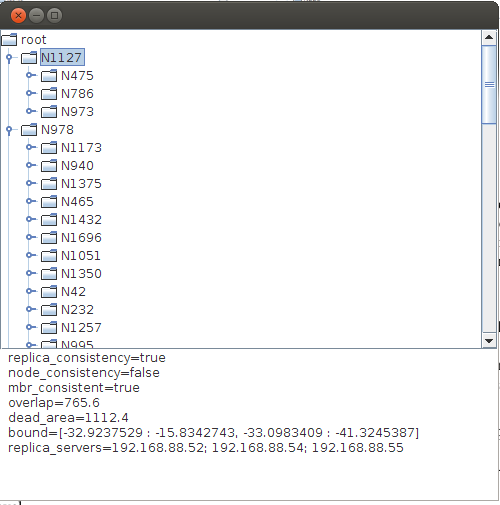
\includegraphics[width=0.45\textwidth]{node_inconsistency.png}
  \label{fig:node_inconsistency}
  } \qquad
  \subfigure[Bound inconsistency]
  {
  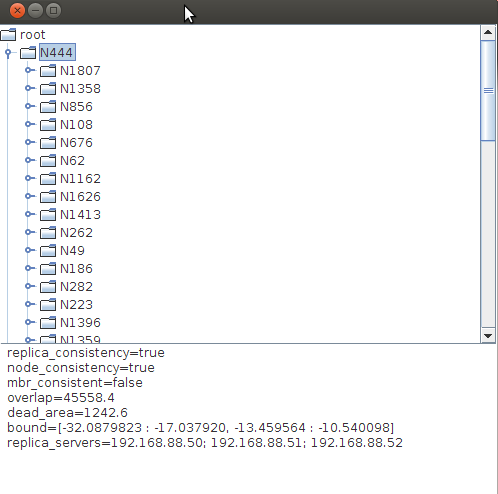
\includegraphics[width=0.45\textwidth]{bound_inconsistency.png}
  \label{fig:bound_inconsistency}
  }
  \caption{RDebug algorithm on business listings dataset}
  \label{fig:rdebug_pois}
\end{figure}

Figure \ref{fig:rdebug_pois} shows the result of RDebug algorithm with the business listings dataset in RDebug Visualizer tool. 
An example of node inconsistency is shown in Figure \ref{fig:node_inconsistency}, which the R-Tree node \textit{N1127} contains only three entries.
This number of entries violates the $m$ value presented in Section \ref{sec:spatial_dist}.
Figure \ref{fig:bound_inconsistency} shows the bound inconsistency between node \textit{N444} and one of its children.
The duplicated nodes identified on R-Tree are shown on final report by RDebug algorithm. 
The user can traverse the R-Tree path on RDebug Visualizer to identify these duplicated nodes.